\section{Benchmarking pathway analysis methods}

With description of the characteristics of existing pathway analysis review papers mentioned in the previous section, we propose a comprehensive framework for benchmarking pathway analysis methods that would tackle the limitations and shortcomings of the previous review papers.

Here we introduce two completely objective, reproducible, and scientifically sound approaches to benchmark pathway analysis methods. In the first sub-section, we evaluate the methods based on their ability to identify the involved phenotypes using real human and mouse benchmark data sets. The second sub-section assesses their performances under the true null hypothesis, i.e. there is no true phenotype involved.

\subsection{Systematic assessment of the methods using benchmark data sets}

%While some of the review papers discuss the theory aspects of the benchmarking methods or use simulated data sets, very few papers compare the methods using small set of benchmarking data sets with limited number of conditions. 

All   data sets were downloaded from Gene Expression Omnibus database. We normalized them using RMA background adjustment, quantile normalization, and median polish summarization.  We used the \textit{threestep} function from \textit{affyPLM} package to perform those steps. Subsequently, standard genome wide annotation packages corresponding to the platform, e.g. hgu133a.db for HG-U133A, were used to map probes to genes. In case there are multiple probes mapped to the same gene, the median value is chosen.

We included 13 methods in this benchmarking study. Eight of these are non-TB methods: Fisher's Exact Test \cite{Fisher:1951}, Kolmogorov-Smirnov test \cite{massey1951kolmogorov}, Wilcoxon Rank Sum test \cite{wilcoxon1945individual}, GSA \cite{Efron:2007}, PADOG \cite{Tarca2012down}, and GSEA \cite{Subramanian:2005}. The other five of them are TB methods: SPIA \cite{SPIAversion2.14.0}, ROntoTools \cite{RontoToolsVersion1.2.0}, CePaGSA, CePaORA \cite{gu2012centrality, gu2013cepa}, and PathNet \cite{Dutta:2012}. We provide details of 13 methods that we would do the benchmarking study in Table~\ref{table:PAmethods}. 

\begin{table}

\centering
\caption{Pathway analysis methods investigated in this study. Versions of KEGG of CePa methods are unknown because they are embedded in the software\label{table:PAmethods}} 
\small
\begin{tabular}{@{}clllll@{}}\hline
 & Method & Category  & R-function/package version & Pathway database \\\hline
1 & Fisher's Exact Test &	non-TB 	& fisher.test & KEGG v.65\\ 
2 & WebGestalt &	non-TB 	& WebGestaltR 0.3.1 & KEGG v.65\\ 
3 & GOstats &	non-TB 	&2.48.0 & KEGG v.65\\ 
4 & Kolmogorov-Smirnov Test& non-TB & ks.test & KEGG v.65\\
5 & Wilcoxon rank sum	& non-TB 	& wilcox.test &  KEGG v.65\\
6 & GSEA &	non-TB & 1.0 & KEGG v.65\\
7 & GSA &	non-TB & 1.03 & KEGG v.65\\
8 & PADOG &	non-TB & 1.20.0 & KEGG v.65\\
9 & SPIA &	TB  & 2.30.0 & KEGG v.65\\
10 & ROntoTools &		TB & 2.6.0 & KEGG v.65\\
11 & CePaORA &	TB & 0.5 & KEGG (version unknown)\\
12 & CePaGSA &	TB & 0.5 & KEGG (version unknown)\\
13 & PathNet &	TB & 1.18.0 & KEGG v.56\\
\hline
\multicolumn{5}{l}{\textit{non-TB}: non topology-based method, \textit{TB}: topology-based method}

\end{tabular}
\end{table}


\subsubsection{Ability to identify the target pathways on human data sets}

One of the most straightforward ways of validating a pathway analysis method is assessing its ability to identify the target pathway describing the related mechanism of the condition studied. 
This validation approach works as follows. First, data sets related to  conditions that already have an associated KEGG pathway (i.e. target pathway) are collected. For each experiment, a perfect method would be able to identify the target pathway as significantly impacted and rank it on top. The target pathway is chosen in advance without human interpretation. Hence, this validation is completely objective and scientifically sound. We apply each method on each of those data sets and report the ranks and p values of target pathways (Fig \ref{workflow}).

\begin{figure}
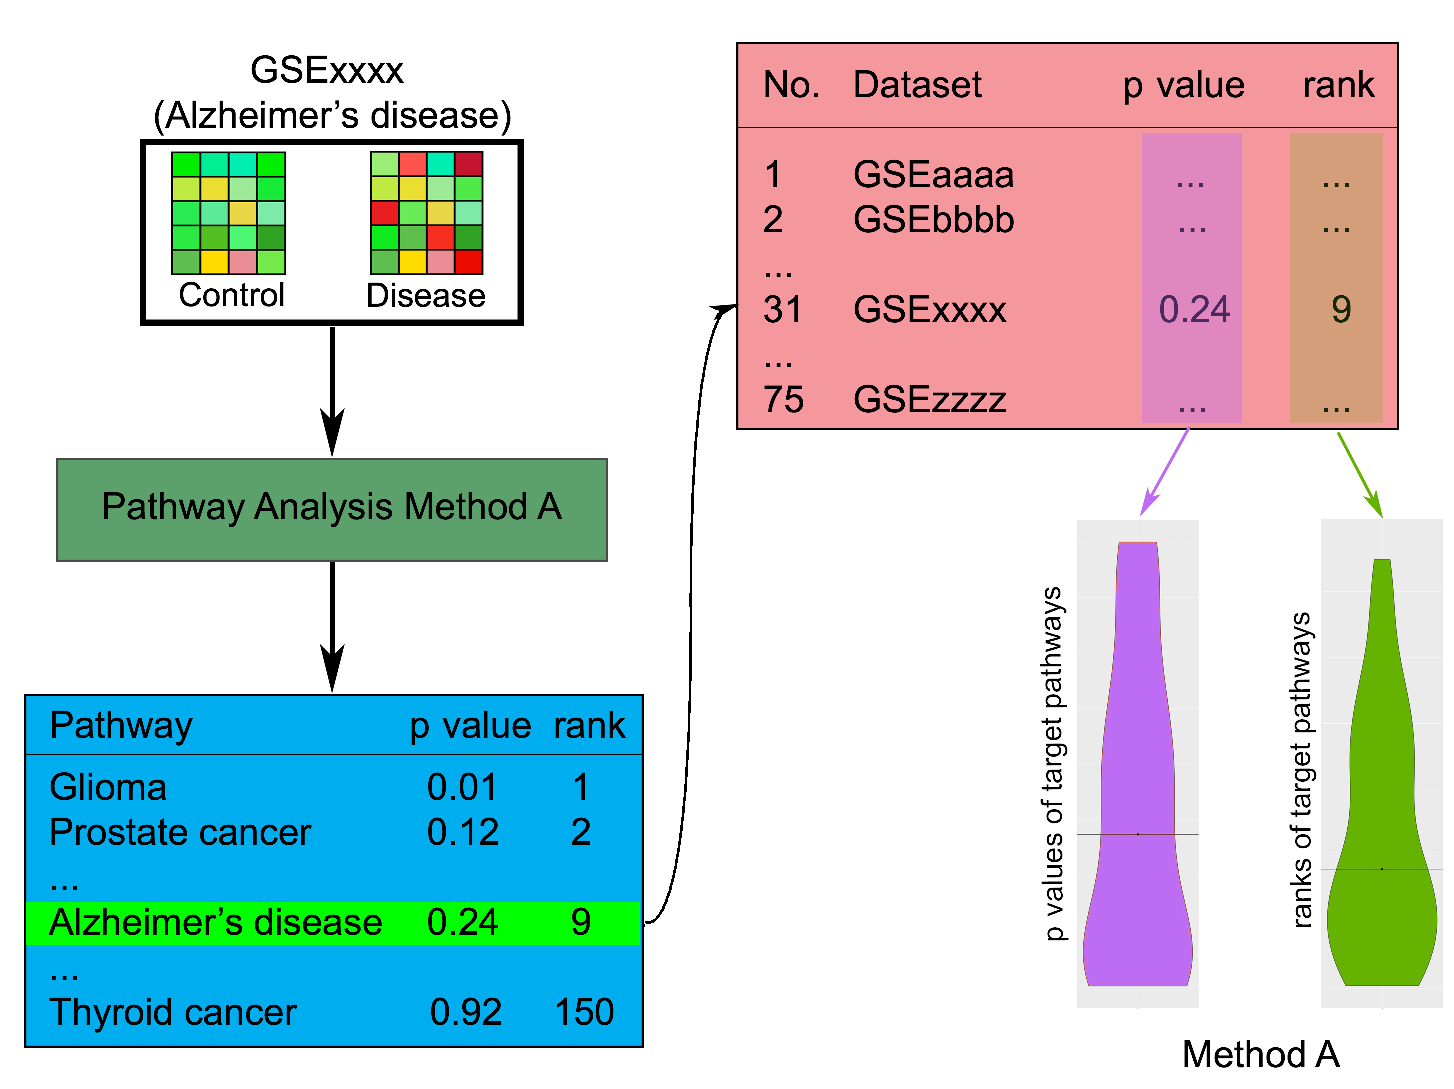
\includegraphics[width=0.8\linewidth]{../Figures/Fig1}
\caption{\textbf{The process of evaluating a pathway analysis method based on their ability to identify target pathways.} Each pathway analysis method is applied on 75 data sets. Methods are evaluated based on their ability to rank the target pathways. In this example, a data set of Alzheimer's disease is examined, and thus the target pathway is ``Alzheimer's disease". Each method produces lists of ranks and p values of the target pathways, which are then used to assess its performance.}
\label{workflow}
\end{figure}

We also take the bias of the methods towards some conditions into consideration. To make it even fairer competition, we choose the same number of data sets per conditions. In fact, we choose 15 widely studied conditions, and 5 data sets per conditions. In total, we used 75 data sets for this study.

Table \ref{table:HumanDatasets} provides detailed information regarding the 75 human data sets used for benchmarking methods' ability to identify target pathways. This information includes: GEO ID, disease, number of normal samples and phenotype samples,  Pubmed ID, tissue from which the samples were taken, and the platform used for the experiment.

\begin{landscape}
\setlength\LTleft{0pt}            % default: \parindent
\setlength\LTright{0pt}           % default: \fill

\centering
\footnotesize
\begin{longtable}{lp{4cm}cccp{4cm}l}
\caption{75 benchmark data sets of 15 diseases used to compare 11 methods in this paper.}\\
\hline
 \textbf{GEO ID}& \textbf{Disease/Condition} & \textbf{\#Normal} & \textbf{\#Condition} & \textbf{Pubmed ID} & \textbf{Tissue} & \textbf{Platform}  \\
 \hline
GSE781 & Renal cell carcinoma	& 5	& 12	& 14641932 &	Kidney &	HG-U133A \\
GSE14762	&Renal cell carcinoma	&12	&9	&19252501	&Kidney	&HG-U133Plus 2.0 \\
GSE6357	&Renal cell carcinoma	&12	&6	&27063186	&CD8+ T Cell	&HG-U133A\\
GSE6344	&Renal cell carcinoma	&10	&10	&17699851	&Clear cell RCC	&HG-U133A\\
GSE48352	&Renal cell carcinoma	&8	&24	&NA	&Kidney	&HG-U133Plus 2.0\\
GSE1297	&Alzheimer’s disease	&9	&7	&14769913	&Hippocampal CA1	&HG-U133A\\
GSE5281EC	&Alzheimer’s disease	&13	&10	&17077275	&Brain, Entorhinal Cortex	& HG-U133Plus 2.0\\
GSE5281HIP	&Alzheimer’s disease	&13	&10	&17077275	&Brain, hippocampus	& HG-U133Plus 2.0\\
GSE5281VCX&	Alzheimer’s disease	&12	&19	&17077275	&Brain, primary visual cortex	& HG-U133Plus 2.0\\
GSE16759	&Alzheimer’s disease&	8	&4	&20126538	&Parietal lobe	&HG-U133Plus 2.0\\
GSE3467&	Thyroid cancer	&9	&9	&16365291	&Thyroid	&HG-U133Plus 2.0\\
GSE3678	&Thyroid cancer	&7	&7	&NA	&Thyroid	&HG-U133Plus 2.0\\
GSE58545	&Thyroid cancer	&18	&27	&26625260	&Thyroid	&HG-U133A\\
GSE85457	&Thyroid cancer	&3	&4	&NA	&Thyroid	&HG-U133Plus 2.0\\
GSE58689	&Thyroid cancer	&18	&27	&26625260	&Thyroid	&HG-U133A\\
GSE3585	&Dilated cardiomyopathy	&5	&7	&17045896	&Heart, subendocardial left ventricular	&HG-U133A\\
GSE33970	&Dilated cardiomyopathy	&18	&5	&NA	&Whole blood and heart	&HG-U133Plus 2.0\\
GSE29819	&Dilated cardiomyopathy	&12	&14	&22085907	&Heart, left and right ventricular	&HG-U133Plus 2.0\\
GSE79962	&Dilated cardiomyopathy	&11	&9	&NA	&Heart	&HuGene-10st\\
GSE21610	&Dilated cardiomyopathy	&8	&42	&20460602	&Heart	&HG-U133Plus 2.0\\
GSE4107	&Colorectal cancer	&10	&12	&17317818	&Colonic mucosa	&HG-U133Plus 2.0\\
GSE8671	&Colorectal cancer	&32	&32	&18171984	&Colon	&HG-U133Plus 2.0\\
GSE9348	&Colorectal cancer	&12	&70	&20143136	&Colon	&HG-U133Plus 2.0\\
GSE23878	&Colorectal cancer	&19	&19	&21281787	&Colon	&HG-U133Plus 2.0\\
GSE4183	&Colorectal cancer	&8	&15	&18776587	&Colon	&HG-U133Plus 2.0\\
GSE6956C	&Prostate cancer	&11	&36	&18245496	&Prostate	&HG-U133A 2\\
GSE6956AA	&Prostate cancer	&7	&33	&18245496	&Prostate	&HG-U133A 2\\
GSE55945	&Prostate cancer	&7	&12	&19737960	&Prostate	&HG-U133Plus 2.0\\
GSE26910	&Prostate cancer	&6	&6	&21611158	&Prostate	&HG-U133Plus 2.0\\
GSE104749	&Prostate cancer	&4	&4	&NA	&Prostate	&HG-U133Plus 2.0\\
GSE8762	&Huntington’s disease	&10	&12	&17724341	&Lymphocyte	&HG-U133Plus 2.0\\
GSE24250	&Huntington’s disease	&6	&8	&21969577	&Venous cellular whole blood	&HG-U133A\\
GSE73655	&Huntington’s disease	&7	&13	&26756592	&Subcutaneous adipose	&HuGene-10st\\
GSE45516	&Huntington’s disease	&3	&6	&24296361	&Fibroblasts	&HG-U133Plus 2.0\\
GSE37517	&Huntington’s disease	&5	&8	&22748968	&Neural stem cell	&HuGene-10st\\
GSE9476	&Acute Myeloid Leukemia	&37	&26	&17910043	&Peripheral blood, bone marrow	&HG-U133A\\
GSE14924\_CD4	&Acute Myeloid Leukemia&	10	&10	&19710498	&CD4 T Cell	&HG-U133Plus 2.0\\
GSE14924\_CD8	&Acute Myeloid Leukemia		&11	&10	&19710498	&CD8 T Cell	&HG-U133Plus 2.0\\
GSE92778	&Acute Myeloid Leukemia	&6	&6	&29035359	&Bone marrow stroma cells	&HuGene-10st\\
GSE68172	&Acute Myeloid Leukemia	&5	&72	&NA	&LSC, HSC and leukemic bulk AML \textsuperscript{*}	&HG-U133Plus 2.0\\
GSE15471	&Pancreatic cancer	&35	&35	&19260470	&Pancreas	&HG-U133Plus 2.0\\
GSE16515	&Pancreatic cancer	&15	&15	&19732725	&Pancreas	&HG-U133Plus 2.0\\
GSE32676	&Pancreatic cancer	&7	&25	&22261810	&Pancreas		&HG-U133Plus 2.0\\
GSE28735	&Pancreatic cancer	&45	&45	&23918603	&Pancreas		&HuGene-10st\\
GSE18670	&Pancreatic cancer	&6	&18	&23157946	&Pancreas	&HG-U133Plus 2.0\\
GSE18842	&Non-small cell lung cancer	&44	&44	&20878980	&Lung	&HG-U133Plus 2.0\\
GSE19188	&Non-small cell lung cancer	&62	&91	&20421987	&Lung	&HG-U133Plus 2.0\\
GSE19804	&Non-small cell lung cancer	&60	&60&	20802022	&Lung	&HG-U133Plus 2.0\\
GSE50627	&Non-small cell lung cancer	&6	&9	&25881239	&Lung	&HuGene-10st\\
GSE6044	&Non-small cell lung cancer	&5	&31	&18992152	&Lung	&HG-Focus\\
GSE19728	&Glioma	&4	&17	&21836821	&Brain	&HG-U133Plus 2.0\\
GSE21354	&Glioma	&4	&13	&21836821	&Brain	&HG-U133Plus 2.0\\
GSE50161	&Glioma	&13	&95	&24078694	&Brain	&HG-U133Plus 2.0\\
GSE4290	&Glioma	&23	&157	 & 16616334	&Brain	&HG-U133Plus 2.0\\
GSE44971	&Glioma	&9	&49	&23660940	&Brain	&HG-U133Plus 2.0\\
GSE20153	&Parkinson’s disease	&8	&8	&20926834	&B lymphocytes from peripheral blood	&HG-U133Plus 2.0\\
GSE20291	&Parkinson’s disease	&20	&15	&15965975	&Brain	&HG-U133A\\
GSE20164	&Parkinson’s disease	&5	&6	&20926834	&Substantia nigra (midbrain)	&HG-U133A\\
GSE7621	&Parkinson’s disease	&9	&16	&17571925	&Substantia nigra (midbrain)	&HG-U133Plus 2.0\\
GSE19587	&Parkinson’s disease	&10	&12	&20837543	&Brain	&HG-U133A 2\\
GSE19420	&Type II diabetes mellitus	&12	&12	&22802091	&Skeletal muscle vastus lateralis	&HG-U133Plus 2.0\\
GSE39825	&Type II diabetes mellitus	&6	&4	&23919306	&Fibroblasts (cell culture)	&HG\_U95Av2\\
GSE26887	&Type II diabetes mellitus	&5	&7	&22427379	&Left ventricle	&HuGene-10st\\
GSE21340	&Type II diabetes mellitus	&15	&5	&23919306	&Skeletal muscle	&HG\_U95Av2\\
GSE38642	&Type II diabetes mellitus	&54	&9	&22768844	&Pancreatic islets	&HuGene-10st\\
GSE24739\_G0	&Chronic Myeloid Leukemia	&4	&8	&21436996	&Peripheral blood	&HG-U133Plus 2.0\\

GSE24739\_G1	&Chronic Myeloid Leukemia	&4	&8	&21436996	&Peripheral blood	&HG-U133Plus 2.0 \\
GSE33075	&Chronic Myeloid Leukemia	&18	&9	&22388797	&Bone marrow	&HG-U133Plus 2.0 \\
GSE24739	&Chronic Myeloid Leukemia	&8	&16	&21436996	&Peripheral blood and bone marrow	&HG-U133Plus 2.0\\
GSE1418	&Chronic Myeloid Leukemia	&6	&8	&15618956	&Bone marrow	&HG-Focus\\
GSE7305	&Endometrial cancer	&10	&10	&17640886	&Endometrium/Ovarian tissue	&HG-U133Plus 2.0\\
GSE63678	&Endometrial cancer	&5	&7	&26559525	&Endometrium	&HG-U133A\\
GSE7803	&Endometrial cancer	&10	&31	&17974957	&Cervix and squamous cervical epitheilium	&HG-U133A\\
GSE17025	&Endometrial cancer	&12	&91	&21619611	&Endometrium	&HG-U133Plus 2.0\\
GSE36389	&Endometrial cancer	&7	&13	&NA	&Endometrium	&HG-U133A\\
\hline
\multicolumn{7}{l}{\textsuperscript{*}\footnotesize{Leukemic stem cells (LSC), hematopoietic stem cells (HSCs), and AML bulk cells (CD34+CD38+, CD34-CD38+ and CD34-CD38)}}
\label{table:HumanDatasets}
\end{longtable}
\end{landscape}


Figure~\ref{overview} shows violin plots for the rankings (top panel) and p value (bottom panel) of the 75 target pathways for each of the 13 competing methods. 

\begin{figure} [!t]
        \begin{subfigure}[h]{0.99\textwidth}
                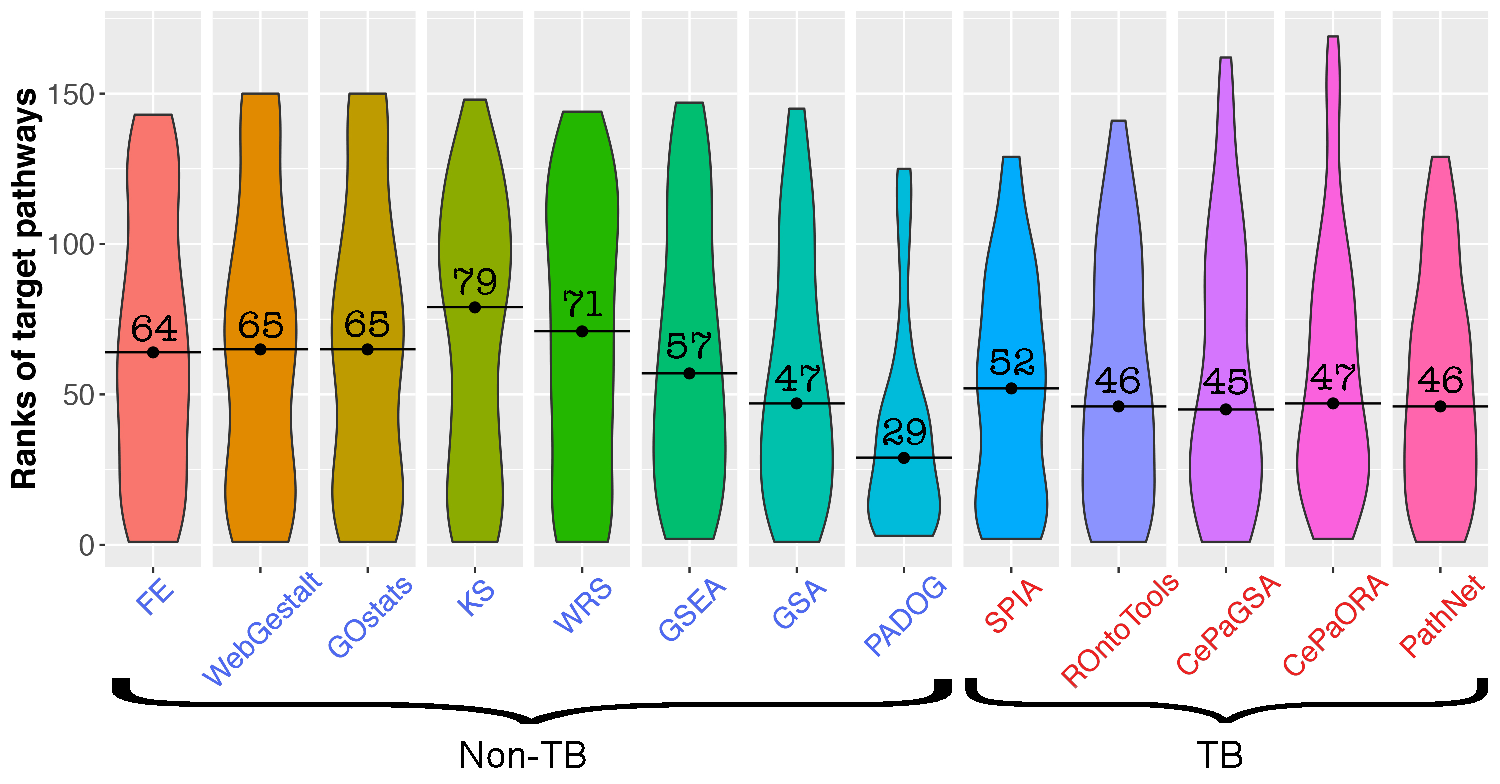
\includegraphics[width=0.98\linewidth]{../Figures/Rank_individual}
                  \caption{Ranks}
                \label{rankCom}
        \end{subfigure}\\
        \begin{subfigure}[h]{0.991\textwidth}
                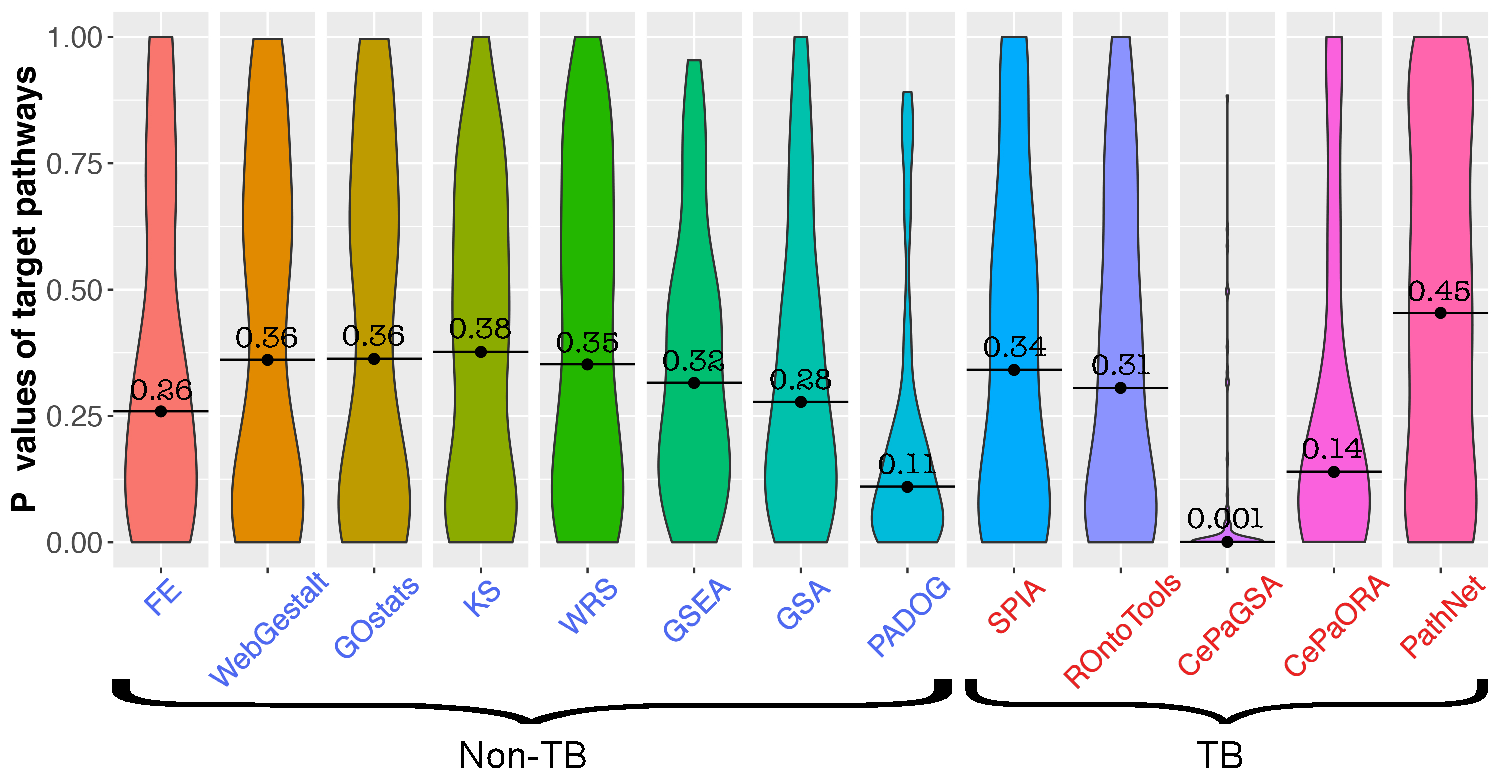
\includegraphics[width=0.98\linewidth]{../Figures/Pvalue_individual}
                \caption{P values}
        \end{subfigure}
        \caption{\textbf{The ranks and p value of target pathways derived by 13 methods.} We perform each method on 75 human benchmark data sets. The resulting ranks and p value of target pathways are plotted in violin plots. The horizontal axis shows the pathway analysis methods in both subfigures. The vertical axis in (\ref{overview}a) represents the ranks while the vertical axis in (\ref{overview}b) corresponds to p value of the target pathways. Hereafter, the labels of non-TB and TB methods are written in blue and red, respectively.}
        \label{overview}
\end{figure}

On a general note, the median rank of target pathways is within the top half for all methods studied, except for KS (Figure~\ref{overview}a). 
None of them, however, has a median rank in the top 20.
Notably, the TB methods are more consistent in ranking the target pathways. 
Specifically, the range of the median rank values obtained by the TB methods (from 45 to 52) is much smaller than the median rank values obtained by the non-TB methods (from 29 to 79). 
Among the non-TB methods, each of the FCS methods (GSEA, GSA and PADOG) performs better than any other methods.

Regarding the performance of the individual methods, the best ranks of target pathways were obtained by PADOG (median rank = 29), followed by CePaGSA, ROntoTools, and PathNet which have median rank values of 45, 46, and 46, respectively. This result also confirms the claims in Tarca \textit{et al.}~\cite{Tarca2012down} that PADOG is better than GSEA and GSA. 

The p value of target pathways using the 13 methods is plotted in Figure \ref{overview}b. In contrast to median ranks, median p value of non-TB methods are comparable to each other while those of TB methods vary considerably.
Among all the methods, the median p value obtained by CePaGSA is the lowest (median p value = 0.001), followed by PADOG (median p value = 0.11) and  CePaORA (median p value = 0.14). 

We also perform a higher level comparison between the ranks and p value of the target pathways obtained by non-TB and TB methods.
As expected, the median rank values of the TB methods are significantly lower (Wilcoxon p value = $8.771\mathrm{E}{-3}$) than those of the non-TB methods (Figure \ref{Fig:nonTBvsTB}a). 
Similarly, the median p value obtained by using TB methods are also significantly lower (Wilcoxon p value = $4.51\mathrm{E}{-4}$) than those of non-TB methods. These results suggest that overall, in this assessment, TB methods are superior to the non-TB methods. 


\begin{figure}
\centering
        \begin{subfigure}[b]{0.3\textwidth}
        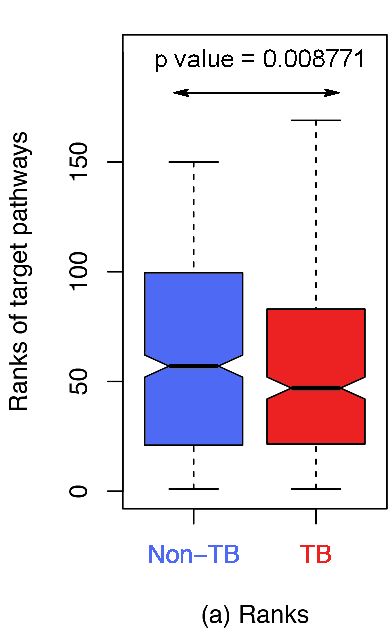
\includegraphics[width=1\linewidth]{../Figures/Ranks_NonTBvsTB}
                \label{rank}
        \end{subfigure}\hspace{10mm}
        \begin{subfigure}[b]{0.3\textwidth}
        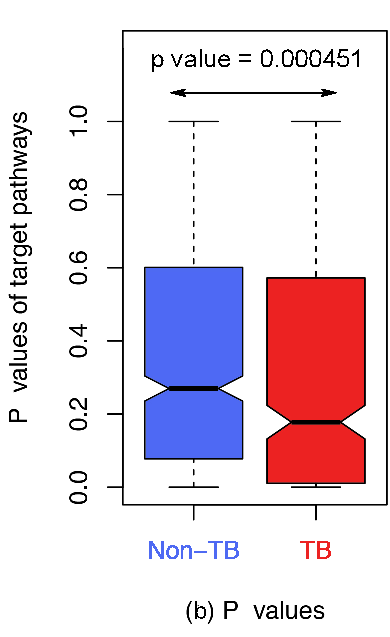
\includegraphics[width=1\linewidth]{../Figures/Pvalue_NonTBvsTB}
                \label{pvalue}
        \end{subfigure}
        \caption{\textbf{The performances of non-TB and TB methods in term of ranks (right panel) and p value (left panel) of target pathways.} We collect all the ranks and p value in Figure \ref{overview} and divide them accordingly into two groups: non-TB and TB methods. Here, lower is better for both ranks and p value.    The  WRS test indicates that TB methods achieved significantly lower ranks (WRS p value = $8.771\mathrm{E}{-3}$) and p value (WRS p value = $4.51\mathrm{E}{-4}$) than those of non-TB methods.}
        \label{Fig:nonTBvsTB}
\end{figure}

%Among the widely used methods described in the previous section, we would choose eleven methods in each groups to perform on real 75 data sets to prepare their individual performances. 

\subsubsection{Ability to identify the pathways containing the cause of the phenotype on mouse data sets}
\label{KOsubsubsection}

Although the above assessment is better than the human interpretation approach or using simulated data sets, it still has some limitations: it focuses solely on one true positive, the target pathway. We do not know what other pathways are also truly impacted and therefore cannot evaluate other criteria such as the accuracy, specificity, sensitivity, and the area under a Receiver Operating Characteristic (ROC) curve (AUC) of a method. Here, we use knock-out data sets that involve using knock-out experiments (KO), where the source of the perturbation is known, i.e. the KO gene.

We use the following inclusion criteria to ensure the quality of KO datasets: (1) The number of samples in a dataset must be at least 4 (at least 2 samples for each genotype), (2) the KO samples must have one and only one KO gene, (3) the KO gene must be in at least one of the pathways in this study, (4) the KO must be differentially expressed, and (5) the expression level of normal samples must be at least three time higher than the expression level of KO samples, i.e the fold-change must be negative and $logFC <= -3$).
We found 13 datasets from GEO satisfied those criteria. Table \ref{table:MouseDatasets} provides detailed information regarding the 13 benchmark KO data sets used. This information includes:  the GEO ID, symbol of KO gene, number of truly impacted pathways, number of normal samples, number of phenotype samples, Pubmed ID, tissue from which the samples were taken, and the platform used for the experiment.


\begin{landscape}
\setlength\LTleft{0pt}            % default: \parindent
\setlength\LTright{0pt}           % default: \fill
\centering
\footnotesize
\begin{longtable}{@{}llcccl@{}}
\caption{Thirteen knockout benchmark data sets used to compare 10 methods in this paper.\label{table:MouseDatasets}}\\
\hline
 \textbf{GEO ID}& \textbf{KO gene} & \textbf{Gene ID}& \textbf{\#Nornal} & \textbf{\#Condition} & \textbf{Known disease association}  \\
 \hline
GSE76669				&Nrf2		&18024	&2	&2	&Cancer, 	neurodegenerative diseases\\
GSE212898\_EGF			&PSEN1		&19164	&3	&3	&Alzheimer’s disease, frontotemporal dementia	\\
GSE212898\_H20			&PSEN1		&19164	&3	&3	&Alzheimer’s disease, frontotemporal dementia	\\	
GSE286963\_NoUVB		&CEBPB		&12608	&4	&4	&Breast cancer, glioblastoma, and lung cancer, obesity\\
GSE286963\_UVB			&CEBPB		&12608	&4	&4	&Breast cancer, glioblastoma, and lung cancer, obesity\\	
%GSE281690				&CNOT3		&232791	&3	&3	&T-cell Acute Lymphoblastic Leukemia, Type 2 Diabetes\\
%GSE285743				&DTX2		&74198	&2	&2	&Neurodevelopmental Disorders, Immune System Disorders\\	
%GSE266662\_OE     			&DLK		&26404	&3	&3	&Metabolic Disorders, Growth and Developmental Disorders\\	
%GSE270482				&NLRX1		&270151	&8	&8	&Autoimmune Diseases, Viral Infections, cancer\\	
GSE50933				&ID3			&15903	&5	&5	&Burkitt Lymphoma, Neurodevelopmental Disorders\\	
GSE62999    				&DUSP5		&240672	&10	&10	&Cardiovascular Diseases, Autoimmune and Inflammatory Diseases\\	
GSE6030    				&NEUROD1	&18012	&3	&3	&Neurodegenerative Diseases, Intellectual Disabilities\\	
%GSE29048    				&PDX1		&18609	&4	&4	&Type 2 Diabetes, Pancreatic Agenesis  \\	
%GSE252926\_Ileum    		&GPR35		&64095	&4	&4	&Inflammatory bowel disease, cancer, cardiovascular diseases\\	
%GSE252926\_macrophage    	&GPR35		&64095	&4	&4	&Inflammatory bowel disease, cancer, cardiovascular diseases \\	
%GSE235163   				&ROCK1		&19877	&3	&3	&Cancer, Fibrotic Diseases,  Cardiovascular Diseases\\	
%GSE195983				&EZR		&22350	&4	&4	&Immune and Inflammatory Diseases, Neurodegenerative Diseases,  \\	
GSE251656\_23C		    	&TXNIP		&56338	&3	&3	&Type 2 diabetes, cardiovascular diseases \\	
GSE251656\_30C			&TXNIP		&56338	&3	&3	&Type 2 diabetes, cardiovascular diseases\\	
GSE280846\_contralateral	&TREM2		&83433	&3	&3	&Alzheimer’s disease,  Nasu-Hakola disease, frontotemporal dementia\\	
GSE280846\_infarction		&TREM2		&83433	&3	&3	&Alzheimer’s disease,  Nasu-Hakola disease, frontotemporal dementia \\	
GSE280846\_peri-infarction	&TREM2		&83433	&3	&3	&Alzheimer’s disease,  Nasu-Hakola disease, frontotemporal dementia\\	
\hline
 \end{longtable}
\end{landscape}

We consider pathways containing the KO gene as positives and the others as negatives. After performing the pathway analysis method on this data set, a p value threshold of 0.05 is used to determine whether a pathway is significantly impacted. A true positive (TP) is a positive which is correctly identified as significant. 
Similarly, a true negative (TN) is a negative which is correctly identified as insignificant.
A false positive (FP) is a pathway that does not contain the KO gene but is reported as significant. A false negative (FN) is a pathway that contains the KO gene but is not reported as significant.

Subsequently, we calculate the accuracy, sensitivity, specificity, and AUC of methods studied using 13 KO data sets.

\textit{Statistical measures} 

With the definitions of true positives (TP), true negatives (TN), false positives (FP), and false negatives (FN) described above, one can calculate the accuracy, sensitivity, and specificity as follows:

\begin{equation}
Accuracy = \frac{TP + TN}{TP + FP + TN + FN}
\end{equation}

\begin{equation}
Sensitivity = \frac{TP}{TP + FN}
\end{equation}
\begin{equation}
Specificity = \frac{TN}{TN + FP}
\end{equation}


The Receiver Operating Characteristic curve (ROC curve) is a graphical representation of the relationship between the sensitivity and the False Positive Rate ($FPR = 1-specificity$) for every possible p value cut-off, where sensitivity is on the y-axis and FPR is on the x-axis. The AUC, the area under the ROC curve, is one of the most important evaluation metrics since it measures a test's discriminative ability.
 

Since CePaGSA, CePaORA, and PathNet do not support mouse pathways, they are left out from these comparisons. 
The comparisons of accuracy, sensitivity, and specificity are illustrated in Fig. \ref{fig:AccSenSpe}.
FE and PADOG have the highest median value of accuracy, 0.92 and 0.91 respectively. PADOG has the highest median value of specificity (0.93), followed by FE (0.92). 
All methods show rather low sensitivity. 
GSA is the best one with the median value of sensitivity of 0.8. 

\begin{figure}
\centering
  \captionsetup{width=0.7\linewidth}

	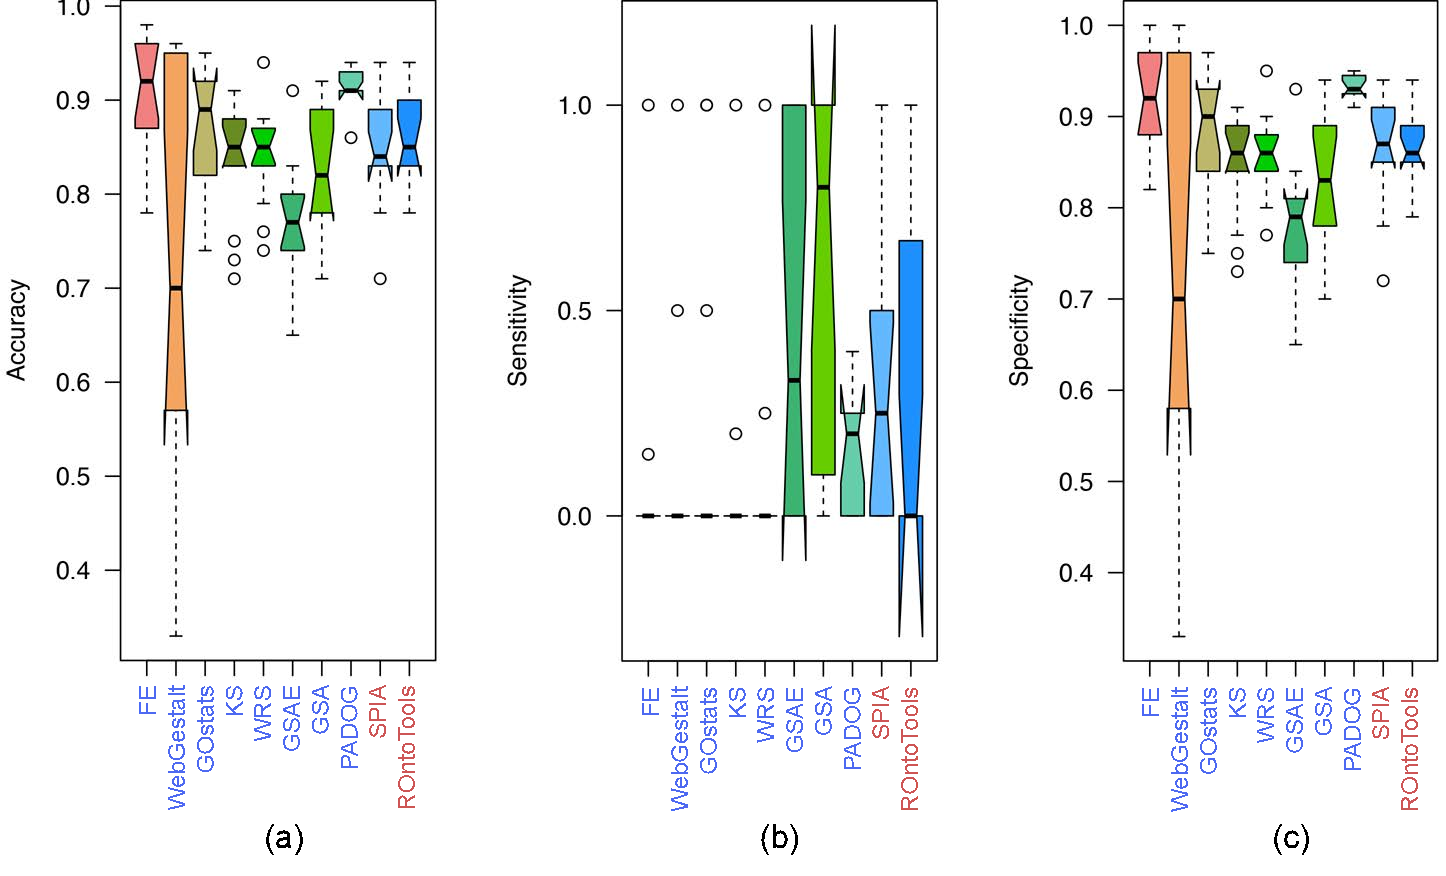
\includegraphics[width=1\linewidth]{../Figures/Acc_Sens_Spec_v3}
	\caption{\textbf{The comparison of 10 methods using KO data sets in term of accuracy (a), sensitivity (b), and specificity (c).} In term of accuracy, FE (0.92) has the highest median value followed by PADOG (0.91). PADOG has the highest median value of specificity (0.93). The best method in term of sensitivity is GSA which has the median value of sensitivity of 0.8 (Fig \label{fig:AccSenSpe}).}
\end{figure}


Among those four statistical measures, the AUC is the most comprehensive and important one because it combines both the sensitivity and specificity across all possible thresholds (Figure \ref{fig:AUC}).
ROntoTools has the highest median value of AUC, namely 0.82, followed by GSA (0.78) and GSEA (0.71).

We also perform a higher level comparison between the ranks and p value of the target pathways obtained by non-TB and TB methods. The AUCs derived by the TB methods (median = 0.7) are higher than those derived by the non-TB methods (median = 0.68) although this superior is not statistically significant (p value = 0.12). 


\begin{figure}
\centering
	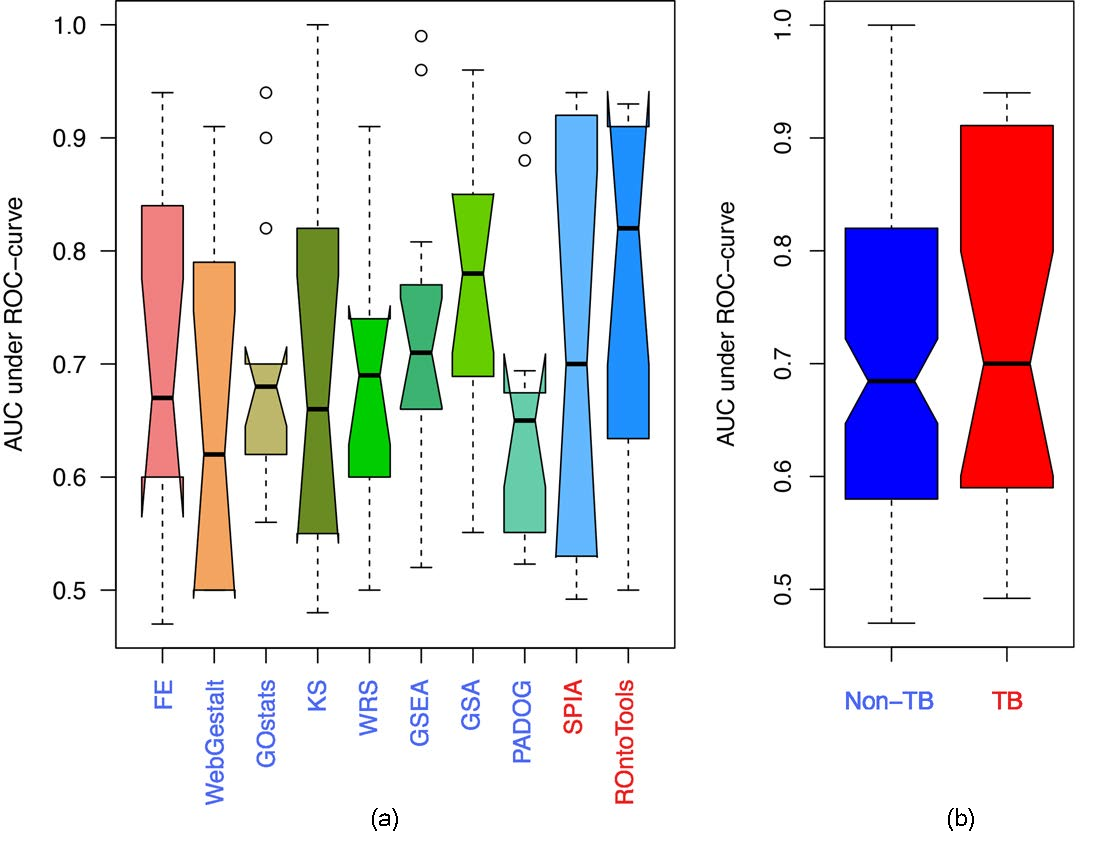
\includegraphics[width=0.8\linewidth]{../Figures/AUC_combined_v3}
  \caption{\textbf{The AUCs of 10 methods using 13 KO data sets (higher is better).} CePaORA, CePaGSA, and PathNet are left out in this comparison because they do not support mouse pathways. ROntoTools has the highest median value of AUC, followed by GSA and GSEA (left panel). Overall, the AUCs obtained by TB methods (0.7) are better than those from non-TB ones (0.68) (right panel). }
  \label{fig:AUC}
\end{figure}




In conclusion, TB methods outperform non-TB methods in all aspects, namely ranks and p value of target pathways, and the AUC. 
Moreover, the results suggest that there is still room for improvement since the ranks of target pathways are still far from optimal in both groups.

\subsection{Investigation of the bias under the null}

In this benchmark, we conduct a deeper investigation into the behavior of these methods under the null hypothesis. 
Here, we create a true null hypothesis by using simulated data sets that are constructed by randomly selected healthy samples from the 75 aforementioned data sets.
We apply each method  more than 2,000 times, each time on different simulated data sets.
Each pathway then has an empirical null distribution of p values resulting from those 2,000 runs (Fig \ref{nullGeneration}).
When the null hypothesis is true, p value obtained from any sound statistical test should be uniformly distributed  between 0 and 1 \cite{barton2013correction, fodor2007towards}.
However, p value generated from many pathway analysis methods are often unimodal (biased toward 0 or 1) or bimodal (biased toward 0 and 1) (Fig. \ref{fig:Biased0} and Fig. \ref{fig:Biased1}). 


\textit{Metric for bias identification}

From all of the non-uniform distributions, we only focus on the ones that are biased toward 0 (right-skewed or positively skewed) or 1 (left-skewed or negatively skewed), since they are responsible for type I and type II errors. We use Pearson's moment coefficient to determine the skewness of a distribution \cite{pearson1895contributions}. It is the third standardized moment and is defined as:

\begin{equation}\label{eq:skewness}
\gamma_1 = E\left[\left(\frac{X-\mu}{\sigma}\right)^3\right] = \frac{\mu_3}{\sigma^3}
\end{equation}

where $\mu$ is the mean, $\sigma$ is the standard deviation, $E$ is the expectation operator, and $\mu_3$ is the third central moment.

If $\gamma_1 \simeq 0$, then the distribution of p values is symmetric, i.e. it is unbiased. 
To decide whether a distribution is biased toward 0 or 1, we set a threshold of $\pm 0.1$.
To be more specific, $\gamma_1 > 0.1$ indicates the distribution is right-skewd (biased toward 0), and $\gamma_1 < -0.1$ means it is left-skewed (biased toward 1).



\begin{figure}
\centering
%  \captionsetup{width=.8\linewidth}

	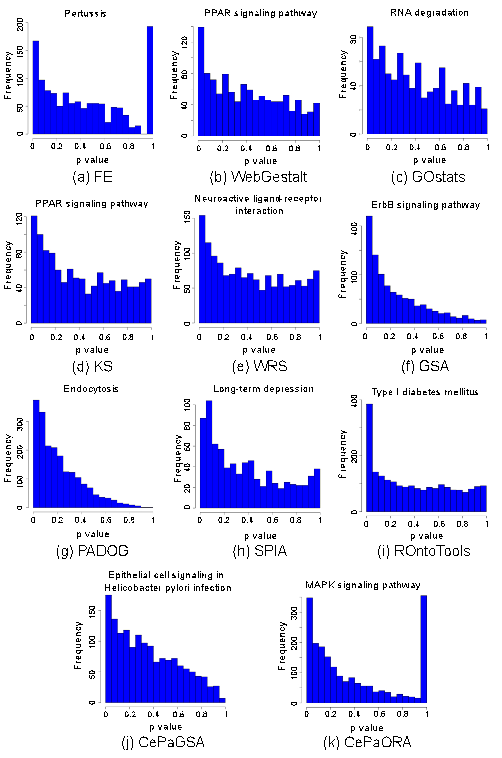
\includegraphics[width=0.8\linewidth]{../Figures/Biased0}
	\caption{\textbf{Examples of pathways that have empirical null distributions of p values biased toward 0.} The procedure for generating null distributions is described in Fig. \ref{nullGeneration}. The x-axes display the p values whereas the y-axes display the frequencies. These pathways are likely to be falsely identified as significantly impacted by the corresponding method (false positive).}\label{fig:Biased0}
\end{figure}

\begin{figure}
\centering
%  \captionsetup{width=.8\linewidth}

	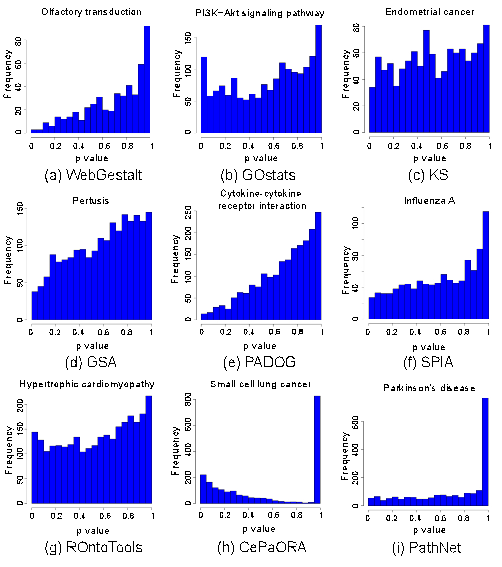
\includegraphics[width=1\linewidth]{../Figures/Biased1}
	\caption{\textbf{Examples of pathways that have empirical null distributions of p values biased toward 1.} In these sub-figures, x-axes represent the p value, while y-axes represent their frequencies. These pathways are often incorrectly excluded in the list of significant pathways  by the corresponding method even when they are indeed impacted (false negative).}\label{fig:Biased1}
\end{figure}


More specifically, a null distribution of p value of a pathway generated by a method skewed to the right (biased toward 0) shows that this method has a tendency to yield low p value and therefore report the pathway as significantly impacted even when it is not (false positive). By contrast, a null distribution of p value of a pathway skewed to the left (biased toward 1) indicates that the given method tends to produce consistently higher p value thus possibly report this pathway as insignificant when it is indeed impacted (false negative).
The results of this null-hypothesis analysis may explain why some methods work well for certain diseases while they perform poorly for others. If a method is biased to report more often a given cancer pathway as significant, that method may be perceived to perform better in experiments involving that particular type of cancer. 

\begin{figure}
\centering
	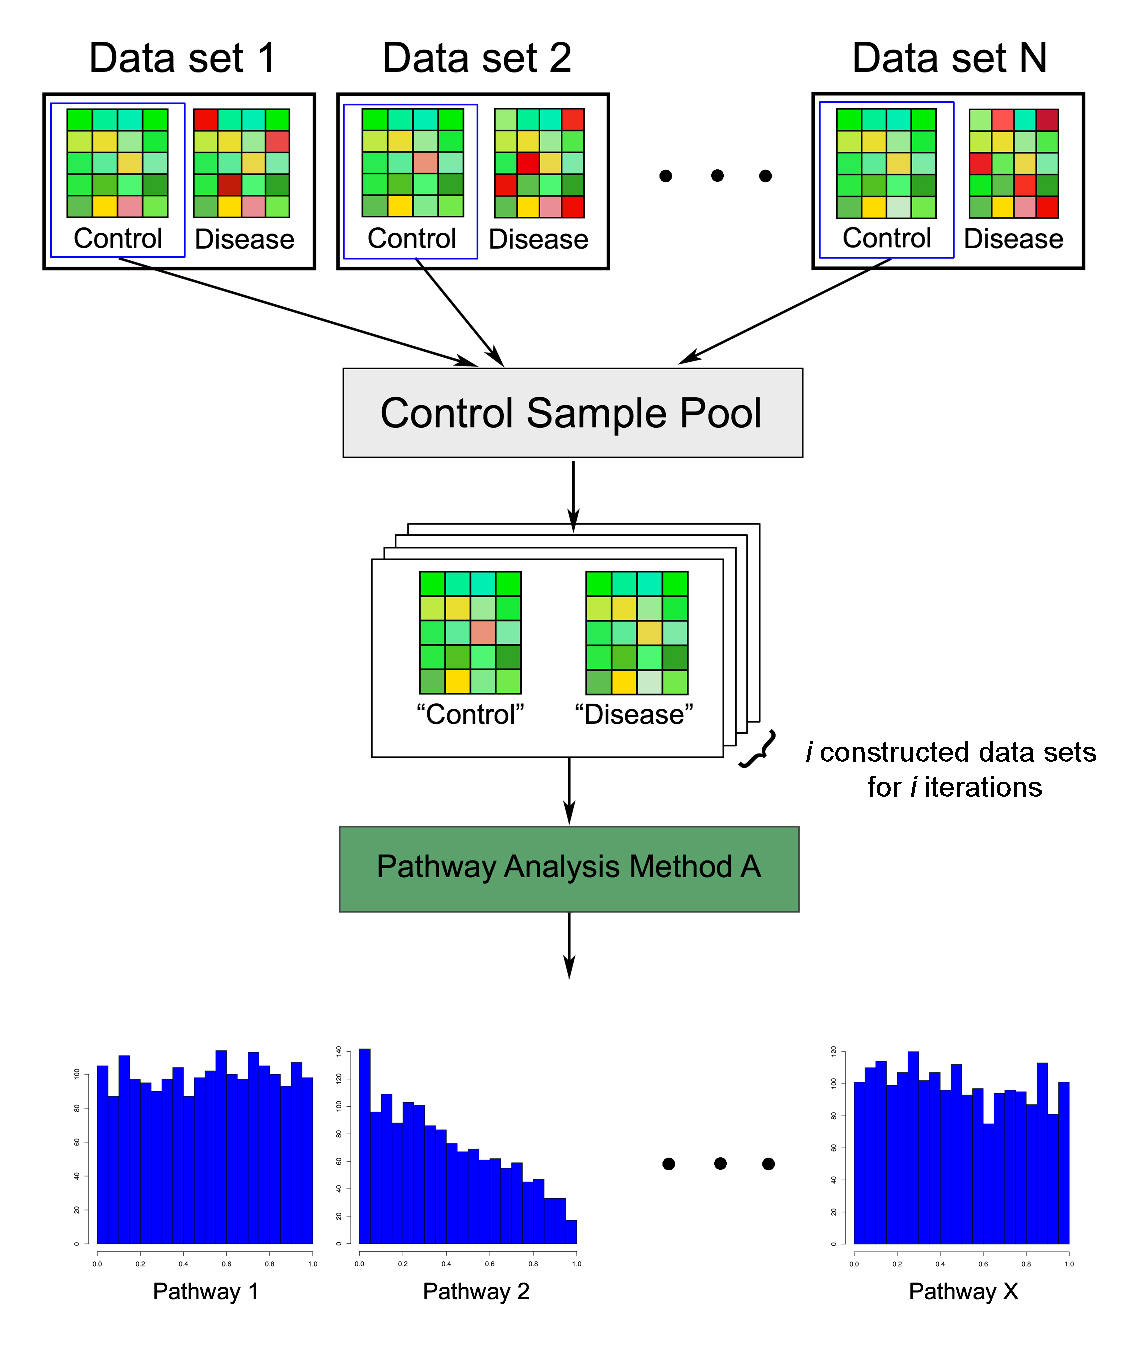
\includegraphics[width=0.8\linewidth]{../Figures/Fig4}
  \caption{\textbf{The process of creating the null distributions of p value for all pathways by a given pathway analysis method.} Control samples from data sets are  gathered to construct a control sample pool. To create the null distribution of p value of all pathways under the null for each method, more than 2,000 iterations were performed. The data sets used in these iterations are generated by randomly selecting samples from the control sample pool.}
  \label{nullGeneration}
\end{figure}

The total number of biased pathways  (either toward 0 or 1) produced by these methods are compared in Figure \ref{fig:NumberOfBias}a.
The number of biased pathways is at least 66 for all the methods compared in this work, except GSEA which has no biased pathway was found. 
While investigating more, we found that the aggregate p value of all the pathways generated by GSEA is uniformly distributed under the null (Fig. \ref{fig:GSEAagg}).
A similar conclusion about GSEA was also reached by Nguyen \textit{et al.}~\cite{nguyen2017DANUBE}.

\begin{figure}
\centering
  \captionsetup{width=.8\linewidth}

	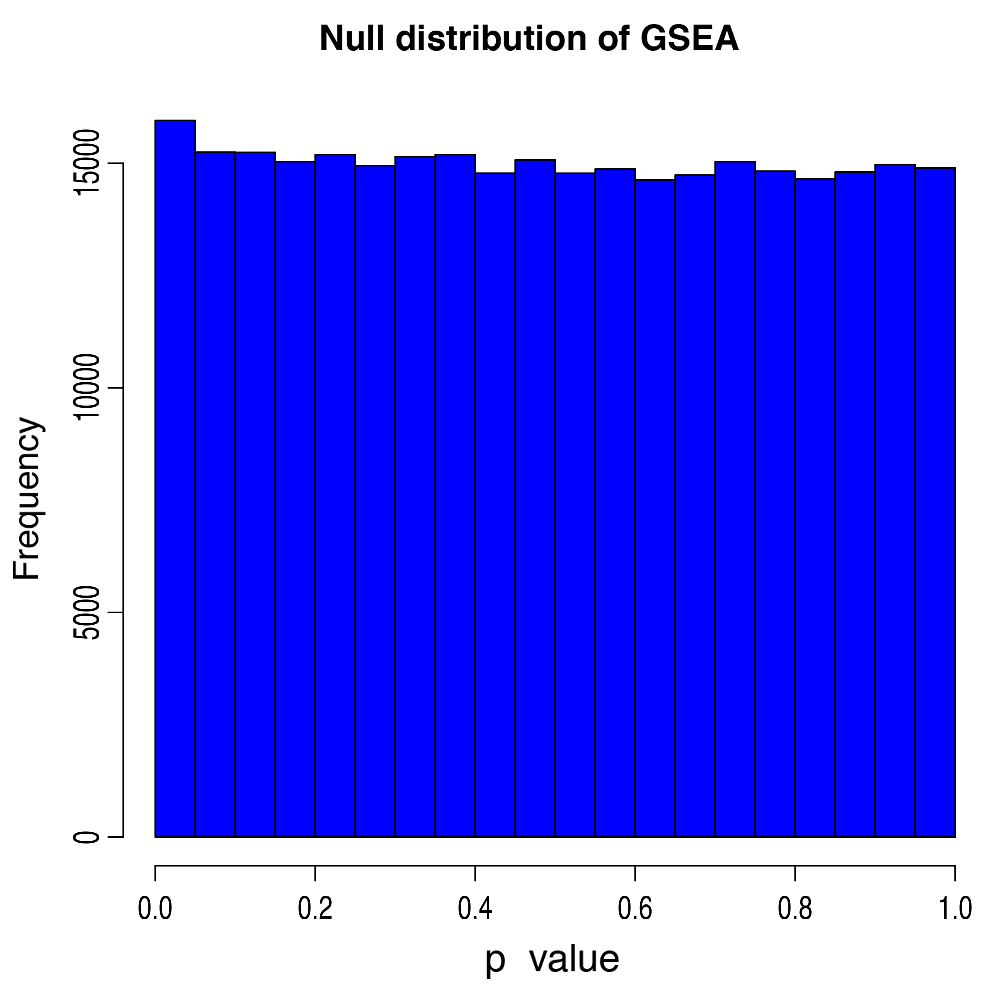
\includegraphics[width=0.5\linewidth]{../Figures/GSEAaggregate}
	\caption{\textbf{Aggregate p values of all the pathways generated by GSEA are uniformly distributed under the null.} The uniform distribution proves that GSEA is extremely unbiased.}\label{fig:GSEAagg}
\end{figure}


The number of pathways biased toward 0 produced by 13 methods are shown in Figure \ref{fig:NumberOfBias}b.
The figure shows that performing pathway analysis using FE test produces the highest number (137 out of 150 pathways) of false positives, this is followed by WRS test (114 out of 150 pathways) and CePaGSA (112 out of 186 pathways). On the other hand, GSEA and PathNet produce no false positive pathways.

Similarly, the numbers of pathways biased toward 1 produced by different methods are shown in Figure \ref{fig:NumberOfBias}c.
PathNet produces the highest number (129 out of 130 pathways) of false negative pathways.
No false negative pathways are identified while performing pathway analysis using GSEA, CePaGSA, WRS test and FE test.

\begin{figure}
\center
	\includegraphics[width=0.7\linewidth]{../Figures/NrBiasedPathway}
        \caption{\textbf{The number of biased pathways calculated based on Pearson's moment coefficient.}  Under the true null hypothesis, an ideal method would produce a uniform distribution of p value from 0 to 1 for every pathway. Here, thresholds of Pearson's moment coefficient of $0.1$ and $-0.1$ are used to determine if the empirical distribution p values is biased toward 0 or 1, respectively.
        Panel (a) shows the total number of biased  pathways (toward either 0 or 1) produced by each method.
Each method, except GSEA, has at least 66 biased pathways.
Panel (b) shows the number of pathways biased toward 0 (false positives) produced by different methods.
FE  produces the highest number (137 out of 150 pathways) of false positives, followed by WRS  (114 out of 150) and CePaGSA (112 out of 186).
Panel (c) shows the number of pathways biased toward 1 (false negatives) produced by different methods.
PathNet produces the highest number (129 out of 130) of false negative pathways. The methods in red are TB methods. The methods in blue are non-TB methods}\label{fig:NumberOfBias}
\end{figure}


\begin{figure}[h]
	\includegraphics[width=0.8\linewidth]{../Figures/NrMethodsBiased}

        \caption{\textbf{The number of methods biased for each pathway.} The y-axis shows the KEGG pathways, while the x-axis indicates the number of methods biased toward 0 and  1, respectively. Each horizontal line represents a pathway. The lengths of the blue and red lines show the number of methods in this study biased toward 0 and 1, respectively. Pathways are sorted by the number of methods biased. There is no pathway that is unbiased for all methods. The top 10 least and top 10 most biased pathways are shown by name.}\label{fig:PathwaysDist}
\end{figure}

\subsection{Discussion}
The goal of pathway analysis is to translate the list of genes that are differentially expressed across the given phenotypes (e.g. disease versus healthy, treated versus non-treated, disease subtype A versus disease subtype B, etc.) into meaningful biological phenomena.
Over the last few years, more than 70 pathway analysis methods have been proposed.
A real problem in the field is the annotation of the pathways. The pathways evolve as more knowledge is gathered. Essentially, at any moment in time, the knowledge captured by the pathways is both incomplete and perhaps partially incorrect. Regardless of the imperfections of today's pathways, one still needs to identify which of these pathways  are significantly impacted in the given phenotype. Hence, extensive benchmarking results will be very useful even though the annotations of the pathway will be imperfect at any one particular time. 
Although there have been already a few publications guiding the users by comparing these methods, they are collectively limited in the following ways: (i) they only discuss the methodological aspects of the methods, (ii) the assessment of the methods are based on simulation data sets which often fail to capture the complexity of real biological phenomena, (iii) they do not compare the performance of the methods under the null, (iv) they do not take into account the systematic bias of a method introduced by the imbalanced number of data sets for one disease, and (v) they do not take the quality of annotation of the pathways into account, which is one of the real challenge in the field.
These limitations may cause significant bias in the conclusions~\cite{nguyen2018network}.
Here, we address all aforementioned issues and provide a systematic assessment and comparison of 13 widely used pathway analysis methods (8 non-TB and 5 TB methods). 
Note that all of the R-packages of the approaches in this study are non-commercial and free for educational purposes. 
Therefore, other popular commercial or web service pathway analysis tools (e.g., iPathwayGuide~\cite{ahsan2017identifying}, Ingenuity Pathway Analysis~\cite{kramer2013causal}, or DAVID~\cite{huang2008systematic}) are out of scope of this review. Nevertheless, the results presented here can be extrapolated to these tools as well, based on the approach used. Thus, iPathwayGuide (www.advaitabio.com) uses the impact analysis that is also implemented in ROntoTools so iPathwayGuide results are expected to be comparable with those of ROntoTools. Also, Ingenuity Pathway Analysis and DAVID are both using a hypergeometric test so their results are expected to be comparable with those obtained with Fisher's Exact test (FE).
 
In order to avoid the potential bias in the comparison, we consider several important factors. 
First, we utilize an equal number of data sets for each disease in our experiment.
This is a crucial factor because if a method tends to unsuccessfully identify some pathways associated with some particular diseases as significantly impacted (type II error), then having too many data sets of these diseases will undermine the rank and the performance of this method.

Second, we attempt to reduce the bias caused by different data sets by selecting a fixed number of DE genes, namely 400 DE genes, for each data set (around 10\% of total number of genes in KEGG).
The classical approach to obtain a list of DE genes from a given gene expression experiment involves applying thresholds based on p value and absolute log-fold changes.
However, due to the heterogeneity present in the individual experiments, the number of DE genes obtained from different studies of the same condition often differ significantly ~\cite{Draghici:2006, tan2003evaluation, ein2005outcome}.
For example, with a threshold for the absolute fold change of 1.5 and a threshold  for corrected p value of 5\%, 21 out of 75 human gene expression data sets studied do not have any DE genes. At the same time,  one of the data sets has more than one thousand DE genes (Fig. \ref{fig:NrDE75}). 
A similar problem occurs with the KO data sets. %, five of which do not have any DE genes according to these criteria (Fig. \ref{fig:NrDEKO}).
This problem in turn makes the downstream analysis (e.g. pathway analysis) inconsistent and biased toward certain data sets. We address this issue by using the same number of DE genes for each data set.

\begin{figure}
\centering
  \captionsetup{width=.6\linewidth}
	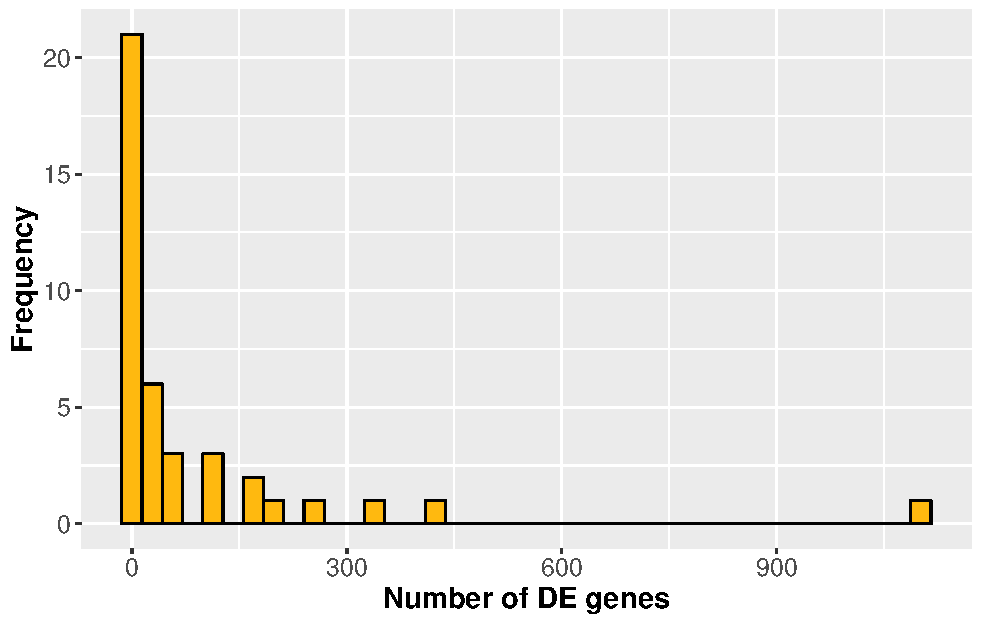
\includegraphics[width=0.6\linewidth]{../Figures/NrDE75}
	\caption{\textbf{The distribution of numbers of DE genes of 75 human gene expression data sets using corrected p value threshold of 0.05 and unsigned log-fold change threshold of 1.5.} The number of DE genes varies considerably across all the data sets. In fact, 21 data sets do not have any DE genes whereas there is one data set that has more than 1000 DE genes.}\label{fig:NrDE75}
\end{figure}

%\begin{figure}
%\centering
%  \captionsetup{width=.6\linewidth}
%
%	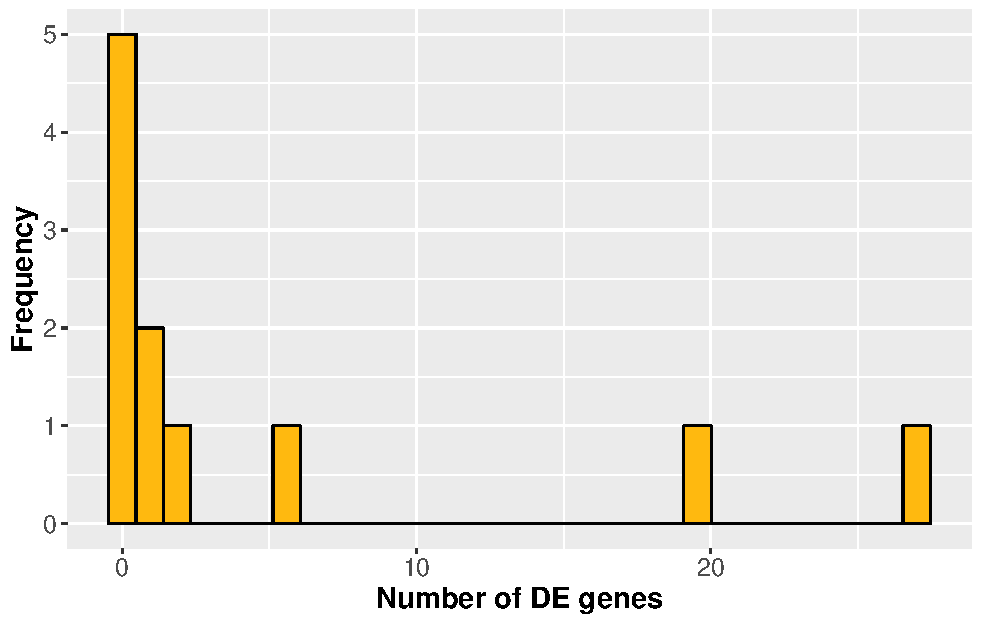
\includegraphics[width=0.6\linewidth]{../Figures/NrDEKO}
%	\caption{\textbf{The distribution of numbers of DE genes of 11 mouse gene expression data sets using corrected p value threshold of 0.05 and unsigned log-fold change threshold of 1.5} Five of them do not have any DE genes.}\label{fig:NrDEKO}
%\end{figure}

In addition, we apply the use of KO data sets in assessing pathway analysis methods, which has never been used in any comparative study in the field.
This approach avoids the shortcoming of the target pathway approach  which focuses on the only one true positive, the target pathway.
However, a knockout is a severe perturbation of a complex organism, and in some sense, most if not all pathways will be affected to some degree.  Given this, the problem becomes philosophical: given that most of all pathways will be affected to some degree, which pathways we want the analysis to identify? Our proposed answer to this is that we want the analysis to identify the pathways that contain the cause of the phenotype, i.e. the KO gene. We feel that this definition is reasonable because it satisfies two conditions: i) all ``interesting'' pathways according to the definition above are truly interesting, and ii) there is no other way to define ``interesting'' pathways without including all other pathways or without using a completely arbitrary decision threshold.

Our assessment using both human and mouse KO data sets shows that the TB methods consistently provide better results than the non-TB methods in terms of ranks and p value of target pathways, as well as the AUC. 

We also evaluate the performances of pathway analysis methods under the null hypothesis.
It is interesting to see that the total number of pathways biased toward 0 is almost double the number of pathways biased toward 1 (696 pathways biased toward 0 versus 356 pathways biased toward 1).
In other words, majority of the pathway analysis methods (except GSEA) tend to consider a given pathway as significantly impacted when it is not truly impacted (i.e. to report false positives). 


More importantly, benchmarking methods based on their performances under the null overcomes the problem of currently poor annotation of the pathways.
In other words, when analyzing two groups of healthy samples (the true null hypothesis) a sound method (e.g. GSEA) should not identify any pathway as significantly impacted regardless its quality of annotation. 

In order to obtain a better understanding of any of these  methods, both studies (the systematic assessment of the methods using benchmark data sets, and the investigation of the bias under the null) performed in this manuscript should be considered.
A method might perform better than other comparative methods in terms of ranks and p value of the target pathways, but that might be due to its intrinsic bias toward 0. 
For example, PADOG achieves the lowest median rank of the target pathways (Figure \ref{overview}a) whereas CepaGSA achieves the lowest median p value (Figure \ref{overview}b).
However, from the second study it appears that an enormous number of the pathways (71 pathways for PADOG, 78 pathways for CePaGSA) reported by these two methods are biased toward 0 (Figure \ref{fig:NumberOfBias}). 
In other words, those low p value are likely to be associated with false positives most of the time. Similarly, GSEA appears to be extremely unbiased, and never yield false positives. However, GSEA  also exhibits a low sensitivity, i.e. a reduced ability to identify the true positives. 

To choose the best pathway analysis method, one should consider the  following four crucial factors in order of importance: (i) \textit{number of biased pathways}, (ii) \textit{ranking of the target pathways}, (iii) \textit{AUC, accuracy, sensitivity, and specificity}, and finally (iv) \textit{p value of the target pathways}. 
The \textit{number of biased pathways} is the most important factor since a less biased method would yield fewer false negatives and fewer false positives in the result.
The second important factor is the \textit{ranking of the target pathways}.
In contrast to the ranking, an assessment of a method based on the derived \textit{p value of the target pathways} is not as trustworthy because the p value are extremely sensitives to these factors. 
For example, the low median p value achieved by CePaGSA is due to the fact that this method reports the majority of the pathways (61.82\% in average) as false positives in any given condition. 

Choosing appropriate data sets is also a very important but often neglected step while benchmarking pathway analysis methods. 
The target pathways related to the diseases or conditions of these data sets should have unbiased null distributions of p value produced by all methods studied. If the null-distribution of p value of a target pathway is not available, knowing the probability of that pathway being biased toward 0 or 1 is also helpful. 
In an attempt to provide this information, for each pathway we calculate the number of methods (out of the 13 methods investigated) biased toward 0 or 1 (Figure \ref{fig:PathwaysDist}). 
The resulting graph indicates that there is no such ``ideal" unbiased pathway.
Each pathway is biased by at least 3 out of 13 investigated methods. 
Some pathways are biased by as many as 12 methods (out of 13 methods).
The common characteristic of these most biased pathways is that they are small in size (less than 50 genes), except for ``PPAR signaling pathway" (259 genes) and ``Complement and coagulation cascades" (102 genes).
In contrast, all pathways in the top 10 least biased have more than 200 genes and up to 2806 genes. In essence, small pathways are generally more likely to be biased than larger ones.
The full list of pathways and their numbers of biased methods is provided in Table \ref{table:NrBiasedMethod}.


\clearpage
\begin{center}
\centering
\footnotesize
\begin{longtable}{@{}ccccc@{}}
\caption{The number of methods biased for each pathway\label{table:NrBiasedMethod}}\\
\hline
 \textbf{Pathway ID}& \textbf{Pathway Names} & \textbf{Bias 0} & \textbf{Bias 1} & \textbf{Total} \\
 \hline
hsa04390	&Hippo signaling pathway&	3&	0&	3\\
hsa04066	&HIF-1 signaling pathway&	3&	0&	3\\
hsa04530	&Tight junction&	3&	1&	4\\
hsa05166	&HTLV-I infection&	5&	0&	5\\
hsa04670	&Leukocyte transendothelial migration&	5&	0&	5\\
hsa05142	&Chagas disease (American trypanosomiasis)&	4&	1&	5\\
hsa04514	&Cell adhesion molecules (CAMs)&	4&	1&	5\\
hsa04310	&Wnt signaling pathway&	4&	1&	5\\
hsa04151	&PI3K-Akt signaling pathway&	4&	1&	5\\
hsa05034	&Alcoholism&	2&	3&	5\\
hsa05169	&Epstein-Barr virus infection&	6&	0&	6\\
hsa05215	&Prostate cancer&	5&	1&	6\\
hsa05212	&Pancreatic cancer&	5&	1&	6\\
hsa05202	&Transcriptional misregulation in cancer&	5&	1&	6\\
hsa05161	&Hepatitis B&	5&	1&	6\\
hsa05030	&Cocaine addiction&	5&	1&	6\\
hsa04810	&Regulation of actin cytoskeleton&	5&	1&	6\\
hsa04726	&Serotonergic synapse&	5&	1&	6\\
hsa04713	&Circadian entrainment&	5&	1&	6\\
hsa04540	&Gap junction&	5&	1&	6\\
hsa04370	&VEGF signaling pathway&	5&	1&	6\\
hsa04270	&Vascular smooth muscle contraction&	5&	1&	6\\
hsa04064	&NF-kappa B signaling pathway&	5&	1&	6\\
hsa05203	&Viral carcinogenesis&	4&	2&	6\\
hsa05164	&Influenza A&	4&	2&	6\\
hsa05162	&Measles	&4&	2&	6\\
hsa05152	&Tuberculosis&	4&	2&	6\\
hsa05120	&Epithelial cell signaling in Helicobacter pylori infection&	4&	2&	6\\
hsa04916	&Melanogenesis&	4&	2&	6\\
hsa04727	&GABAergic synapse&	4&	2&	6\\
hsa04723	&Retrograde endocannabinoid signaling&	4&	2&	6\\
hsa04330	&Notch signaling pathway&	4&	2&	6\\
hsa04210	&Apoptosis&	4&	2&	6\\
hsa03460	&Fanconi anemia pathway&	4&	2&	6\\
hsa04920	&Adipocytokine signaling pathway&	3&	3&	6\\
hsa04144	&Endocytosis&	3&	3&	6\\
hsa04914	&Progesterone-mediated oocyte maturation&	7&	0&	7\\
hsa05214	&Glioma&	6&	1&	7\\
hsa05168	&Herpes simplex infection&	6&	1&	7\\
hsa04725	&Cholinergic synapse&	6&	1&	7\\
hsa04724	&Glutamatergic synapse&	6&	1&	7\\
hsa04721	&Synaptic vesicle cycle&	6&	1&	7\\
hsa04664	&Fc epsilon RI signaling pathway&	6&	1&	7\\
hsa04380	&Osteoclast differentiation&	6&	1&	7\\
hsa04360	&Axon guidance&	6&	1&	7\\
hsa05323	&Rheumatoid arthritis&	5&	2&	7\\
hsa05218	&Melanoma&	5&	2&	7\\
hsa05210	&Colorectal cancer&	5&	2&	7\\
hsa05132	&Salmonella infection&	5&	2&	7\\
hsa04340	&Hedgehog signaling pathway&	5&	2&	7\\
hsa04010	&MAPK signaling pathway&	5&	2&	7\\
hsa03008	&Ribosome biogenesis in eukaryotes&	5&	2&	7\\
hsa05032	&Morphine addiction&	4&	3&	7\\
hsa04620	&Toll-like receptor signaling pathway&	4&	3&	7\\
hsa05016	&Huntington's disease&	3&	4&	7\\
hsa04650	&Natural killer cell mediated cytotoxicity&	3&	4&	7\\
hsa04961	&Endocrine and other factor-regulated calcium reabsorption&	8&	0&	8\\
hsa05222	&Small cell lung cancer&	7&	1&	8\\
hsa05145	&Toxoplasmosis&	7&	1&	8\\
hsa05031	&Amphetamine addiction&	7&	1&	8\\
hsa04912	&GnRH signaling pathway	&7&	1&	8\\
hsa04666	&Fc gamma R-mediated phagocytosis&	7&	1&	8\\
hsa04662	&B cell receptor signaling pathway&	7&	1&	8\\
hsa04350	&TGF-beta signaling pathway&	7&	1&	8\\
hsa05200	&Pathways in cancer&	6&	2&	8\\
hsa05160	&Hepatitis C&	6&	2&	8\\
hsa04520	&Adherens junction&	6&	2&	8\\
hsa05217	&Basal cell carcinoma&	5&	3&	8\\
hsa05134	&Legionellosis&	5&	3&	8\\
hsa05133	&Pertussis&	5&	3&	8\\
hsa05010	&Alzheimer's disease&	5&	3&	8\\
hsa04973	&Carbohydrate digestion and absorption&	5&	3&	8\\
hsa04145	&Phagosome&	5&	3&	8\\
hsa04020	&Calcium signaling pathway&	5&	3&	8\\
hsa05322	&Systemic lupus erythematosus&	4&	4&	8\\
hsa04622	&RIG-I-like receptor signaling pathway&	4&	4&	8\\
hsa04142	&Lysosome&	4&	4&	8\\
hsa05100	&Bacterial invasion of epithelial cells&	8&	1&	9\\
hsa04710	&Circadian rhythm&	8&	1&	9\\
hsa04130	&SNARE interactions in vesicular transport&	8&	1&	9\\
hsa04012	&ErbB signaling pathway&	8&	1&	9\\
hsa03015	&mRNA surveillance pathway&	8&	1&	9\\
hsa05412	&Arrhythmogenic right ventricular cardiomyopathy (ARVC)&	7&	2&	9\\
hsa05223	&Non-small cell lung cancer&	7&	2&	9\\
hsa05220	&Chronic myeloid leukemia&	7&	2&	9\\
hsa05211	&Renal cell carcinoma&	7&	2&	9\\
hsa05130	&Pathogenic Escherichia coli infection&	7&	2&	9\\
hsa04971	&Gastric acid secretion&	7&	2&	9\\
hsa04960	&Aldosterone-regulated sodium reabsorption&	7&	2&	9\\
hsa04910	&Insulin signaling pathway&	7&	2&	9\\
hsa04730	&Long-term depression&	7&	2&	9\\
hsa04728	&Dopaminergic synapse&	7&	2&	9\\
hsa04720	&Long-term potentiation&	7&	2&	9\\
hsa04150	&mTOR signaling pathway&	7&	2&	9\\
hsa04114	&Oocyte meiosis&	7&	2&	9\\
hsa04110	&Cell cycle&	7&	2&	9\\
hsa05416	&Viral myocarditis&	6&	3&	9\\
hsa05332	&Graft-versus-host disease&	6&	3&	9\\
hsa05221	&Acute myeloid leukemia&	6&	3&	9\\
hsa05219	&Bladder cancer&	6&	3&	9\\
hsa05216	&Thyroid cancer&	6&	3&	9\\
hsa05146	&Amoebiasis&	6&	3&	9\\
hsa05143	&African trypanosomiasis&	6&	3&	9\\
hsa05014	&Amyotrophic lateral sclerosis (ALS)&	6&	3&	9\\
hsa04978	&Mineral absorption&	6&	3&	9\\
hsa04940	&Type I diabetes mellitus&	6&	3&	9\\
hsa04621	&NOD-like receptor signaling pathway&	6&	3&	9\\
hsa05410	&Hypertrophic cardiomyopathy (HCM)&	5&	4&	9\\
hsa05140	&Leishmaniasis	&5&	4&	9\\
hsa05012	&Parkinson's disease&	5&	4&	9\\
hsa04970	&Salivary secretion&	5&	4&	9\\
hsa04742	&Taste transduction&	5&	4&	9\\
hsa04630	&Jak-STAT signaling pathway&	4&	5&	9\\
hsa05131	&Shigellosis&	8&	2&	10\\
hsa04722	&Neurotrophin signaling pathway&	8&	2	&10\\
hsa04660	&T cell receptor signaling pathway	&8	&2&	10\\
hsa04512	&ECM-receptor interaction&	8&	2&	10\\
hsa04115	&p53 signaling pathway&	8&	2&	10\\
hsa05213	&Endometrial cancer	&7&	3&	10\\
hsa04950	&Maturity onset diabetes of the young&	7&	3&	10\\
hsa04122	&Sulfur relay system&	7&	3&	10\\
hsa05310	&Asthma&	6&	4&	10\\
hsa04976	&Bile secretion&	6&	4&	10\\
hsa04972	&Pancreatic secretion&	6&	4&	10\\
hsa04612	&Antigen processing and presentation&	6&	4&	10\\
hsa04062	&Chemokine signaling pathway&	6&	4&	10\\
hsa04060	&Cytokine-cytokine receptor interaction&	6&	4&	10\\
hsa05414	&Dilated cardiomyopathy&	5&	5&	10\\
hsa04740	&Olfactory transduction&	5&	5&	10\\
hsa04140	&Regulation of autophagy&	5&	5&	10\\
hsa04962	&Vasopressin-regulated water reabsorption&	9&	2&	11\\
hsa04930	&Type II diabetes mellitus&	9&	2&	11\\
hsa04510	&Focal adhesion&	9&	2&	11\\
hsa05150	&Staphylococcus aureus infection&	8&	3&	11\\
hsa04320	&Dorso-ventral axis formation&	8&	3&	11\\
hsa04141	&Protein processing in endoplasmic reticulum&	8&	3&	11\\
hsa03018	&RNA degradation&	8&	3&	11\\
hsa03013	&RNA transport&	8&	3&	11\\
hsa05330	&Allograft rejection&	7&	4&	11\\
hsa05110	&Vibrio cholerae infection&	7&	4&	11\\
hsa04744	&Phototransduction&	7&	4&	11\\
hsa04672	&Intestinal immune network for IgA production&	7&	4&	11\\
hsa04610	&Complement and coagulation cascades&	7&	4&	11\\
hsa04260	&Cardiac muscle contraction&	7&	4&	11\\
hsa05020	&Prion diseases&	6&	5&	11\\
hsa03320	&PPAR signaling pathway&	6&	5&	11\\
hsa04080	&Neuroactive ligand-receptor interaction&	4&	7&	11\\
hsa05320	&Autoimmune thyroid disease&	7&	5&	12\\
hsa05144	&Malaria&	7&	5&	12\\
hsa04623	&Cytosolic DNA-sensing pathway&	7&	5&	12\\
\hline
 \end{longtable}
\end{center}


\subsubsection{Recommendations for pathway analysis users}
Based on the extensive testing and comparisons described here, we can provide some guidance for researchers who need to perform a pathway analysis. First and foremost, one should decide what type of analysis they are interested in. Topology-based (TB) methods  provide a better ability to identify pathways that contain genes that caused the phenotype or are closely related to it (such as KO genes, or genes bearing variants that significantly affect their function, etc.). A topology-based analysis is also recommended when (i) it is important to consider how various genes interact, (ii) one wishes to take advantage of the sizes and directions of measured expression changes, (iii) one wishes to account for the type and direction of interactions on a pathway, (iv) one intends to predict or explain downstream or pathway-level effects, and (v) one is interested in understanding the underlying mechanisms. The topology-based approach that  provided the best AUC across our 11 KO data set was the impact analysis, as implemented in ROntoTools~\cite{ROntoTools1.2.0}. The same impact analysis approach is also used in  iPathwayGuide~\cite{ahsan2017identifying,Pathway-GuideSoftware}.

A non-TB method may be more useful when one needs to analyze arbitrarily defined sets of genes, rather than pathways. In this category, GSEA provided the highest AUC in our extensive testing. GSEA was also the most un-biased method out of the 13 approaches benchmarked in our studies. 

The Fisher's Exact (FE) test or hypergeometric test is arguably the most widely  used method for enrichment analysis. However,  our results show that FE is not very suitable in the context of pathway analysis. Figure \ref{fig:NumberOfBias} shows that FE test performs the worst among the 13 compared pathway analysis methods:  137 out of 150 pathways are biased toward 0, that being very likely to often produce false positives. This  should be a strong cautionary note to the users of other platforms using this test, such as Ingenuity Pathway Analysis~\cite{kramer2013causal}, or DAVID~\cite{huang2008systematic}.
One of the main reasons for the poor performance of the FE test is that it assumes that the genes are independent, while the genes on any pathway influence each other as described by the pathway. Another reason is that the FE test ignores the roles of genes situated in key positions (e.g. a single entry point in a pathway), as well as the number, direction and type of various signals through which genes on the pathway interact with each other.
